\begin{figure}[bh]
\begin{center}
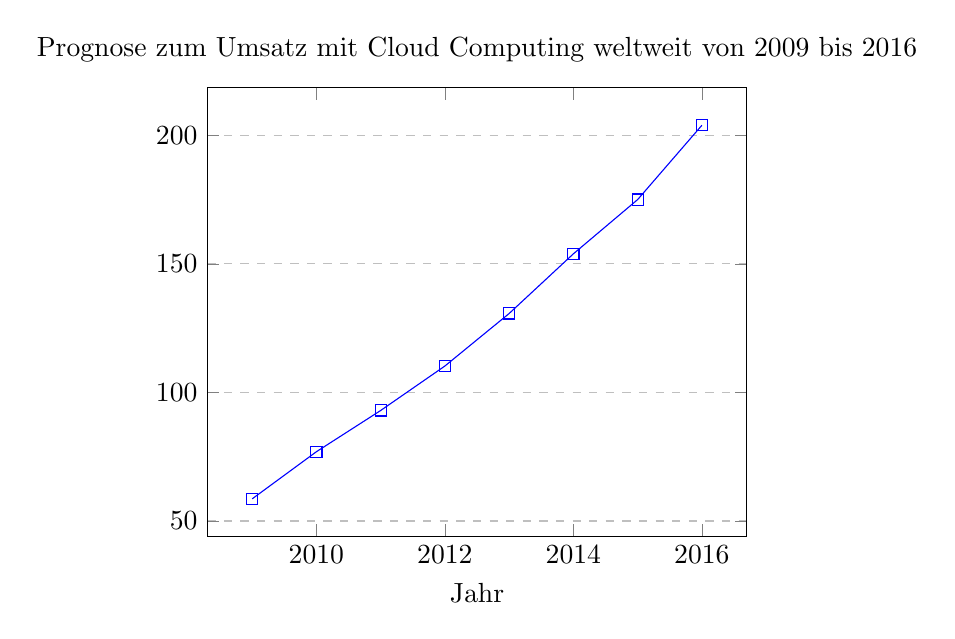
\begin{tikzpicture}
\begin{axis}[
/pgf/number format/.cd,
        use comma,
        1000 sep={},
    title={Prognose zum Umsatz mit Cloud Computing weltweit von 2009 bis 2016},
    xlabel={Jahr},
    %ylabel={Umsatz [Mio. US-Dollar]},
    %xmin=2012, xmax=2016,
    %ymin=0, ymax=8000,
    %xtick={0,20,40,60,80,100},
    %ytick={0,20,40,60,80,100,120},
    legend pos=north west,
    ymajorgrids=true,
    grid style=dashed
]

\addplot[color=blue,mark=square,]
    coordinates {
	(2009,58.6)
	(2010,76.94)
	(2011,92.97)
	(2012,110.27)
	(2013,130.7)
	(2014,153.91)
	(2015,175)
	(2016,203.9)
    };
    %{Cloud Umsatz weltweit}
    
%\addplot[color=green,mark=square,]
%    coordinates {
%    
%(2009,0)(2010,0)(2011,0)(2012,2.267)(2013,3.050)(2014,4.071)(2015,5.374)(2016
% ,6.667)
%    };
    %\legend{Salesforce}
 
\end{axis}
\end{tikzpicture} 
\caption{Prognose zum Umsatz mit Cloud Computing weltweit von 2009 bis 2015 mit 
geschätztem Wert für 2016 entnommen aus \cite{CloudUmsatzWeltweit} }
\label{umsatz_cloud_computing_weltweit}

\end{center}
\end{figure}
